
\documentclass[conference,12pt,letterpaper]{IEEEtran}
\usepackage[margin=1in]{geometry}
\usepackage{array,tabularx}
\usepackage{graphicx,xcolor,float}
\usepackage{cite,balance}
\usepackage[hidelinks]{hyperref}

\renewcommand{\thesection}{\arabic{section}}
\newcolumntype{Y}{>{\raggedright\arraybackslash}X}
\renewcommand{\arraystretch}{1.25}
\urlstyle{same}
\raggedbottom

\title{From Blocks to Behaviors: Teaching Computational Thinking with Reachy Mini\\
\large Final Project Proposal\\
INFO 5356: Introduction to Human-Robot Interaction}

\author{
\IEEEauthorblockN{Elliot Zhang, Jaclyn Pham, Yifan (Fanning) Luo, Jiaxin (Aurora) Shen}
\IEEEauthorblockA{Cornell Tech\\
\{qz432, cqp4, yl4389, js3996\}@cornell.edu}
}

\begin{document}
\maketitle

\section{Proposed Interactive Robotic Game}

\subsection{Project Overview}

Disco Moo is a collaborative, tangible-programming game for groups of 3--4 middle school students. Inspired by Scratch, students connect physical coding blocks to program a cow-themed Reachy Mini. A camera recognizes ArUco markers on the blocks and translates their order into head, body, and antenna movements. Reachy presents short dance challenges, performs the assembled program, and responds with feedback. A group completes a mission when its program matches the target; incorrect attempts can be revised and retried. The activity lasts 5--6 minutes.

\subsection{Learning Objectives}

Students will (1) predict how command order affects behavior (\emph{sequencing}), (2) use loops to express repeated movements (\emph{repetition}), and (3) compare intended and observed actions to locate and correct errors (\emph{debugging}). These concepts build on middle-school block-based programming without requiring text-based coding. A five-teacher K--12 panel (October 28, 2026) recommended progressive tasks, clear instructions, supportive hints, and rotating group roles. After the activity, students should be able to apply these skills to Scratch or introductory programming exercises.

\subsection{Research Questions or Hypotheses}

\textbf{RQ1 (exploratory):} How do students use tangible blocks and visible robot movements to identify and correct sequencing and repetition errors? We will observe error types, revisions, and collaboration.

\textbf{H1 (confirmatory):} Groups receiving specific, encouraging debugging hints will correct a greater proportion of errors than groups receiving neutral mismatch notifications. The independent variable is feedback type; the dependent variable is successful corrections per debugging opportunity. This prediction is motivated by child--robot interaction research and teacher feedback; findings will be preliminary given the short sessions.

\section{Background and Related Work}

\subsection{Literature Search}

Search terms included ``educational robotics,'' ``human-robot interaction,'' ``tangible programming,'' ``computational thinking,'' ``child-robot interaction,'' and ``debugging.'' We prioritized 2022--2026 research in HRI/robotics and related peer-reviewed education venues.

\subsection{Tangible Programming and Embodied Computational Thinking}

Sinha et al.~\cite{paper1} examine how young learners connect physical activity with computational representations; Misirli and Komis~\cite{paper4} study debugging knowledge developed through tangible robots. Both support making program structure observable. However, their younger-child contexts leave open how middle-school groups jointly debug an expressive robot. Disco Moo links three representations---assembled blocks, an on-screen command list, and executed movements---so students can inspect discrepancies.

\subsection{Social Robot Feedback and Educational Engagement}

De Jong et al.~\cite{paper2} investigate how children's acceptance of a social robot changes over time, while Ligthart et al.~\cite{paper3} examine recurring educational child--robot interactions. These studies motivate attention to social feedback but do not directly test task-specific debugging hints in a brief collaborative programming game. Disco Moo addresses this gap by comparing encouraging, actionable hints with neutral notifications while documenting learning-related behavior and robot perceptions.

\section{Methods}

\subsection{Game Design and Assumptions}

Reachy Mini sits at the rear of a tabletop facing 3--4 students, with a visible mission display and a designated block-scanning area (Fig.~\ref{fig:setting}). The camera reads ArUco IDs and spatial order; software maps them to predefined actions and evaluates the resulting program. Students assemble and present blocks, then observe and revise. We assume stable lighting, camera visibility, connectivity, and safe robot motion. Lab 4 validated paper-marker recognition and sequential movement execution; markers on assembled 3D-printed blocks and loop handling still require testing.

\subsection{Game Mechanics}

\textbf{Setting and components.} CODE Farmland includes a cow-costumed Reachy Mini, laser-cut sign, interlocking 3D-printed blocks, ArUco labels, a camera interface, and a laptop showing missions, recognized commands, and feedback.

\textbf{Core actions and progression.} Students plan, assemble, scan, observe, and revise programs through three missions: \emph{(1) Sequencing}, arranging LOOK LEFT, NOD, and LOOK RIGHT in order; \emph{(2) Loops}, expressing repeated movements such as three nods; and \emph{(3) Free Programming}, designing a short original movement sequence. Difficulty progresses from order to repetition to independent application. Debugging occurs throughout rather than as a separate mission.

\textbf{Challenges and rules.} Students must distinguish commands, maintain order, and correct mismatches. Only provided blocks may be scanned; markers must remain visible, and students must not touch the robot while it moves. Reachy executes supported, predefined motions only; it cannot move or rearrange blocks. Incorrect programs can be retried.

\textbf{Robot role and collaboration.} Reachy acts as an encouraging dance partner, introducing missions through screen prompts and sounds, demonstrating movements, celebrating success, and signaling errors with head gestures and hints. Students rotate Planner, Builder, Debugger, and Observer roles (the Observer role is shared in groups of three). The display highlights the current command, connecting physical code with observed motion.

\begin{figure}[H]
\centering
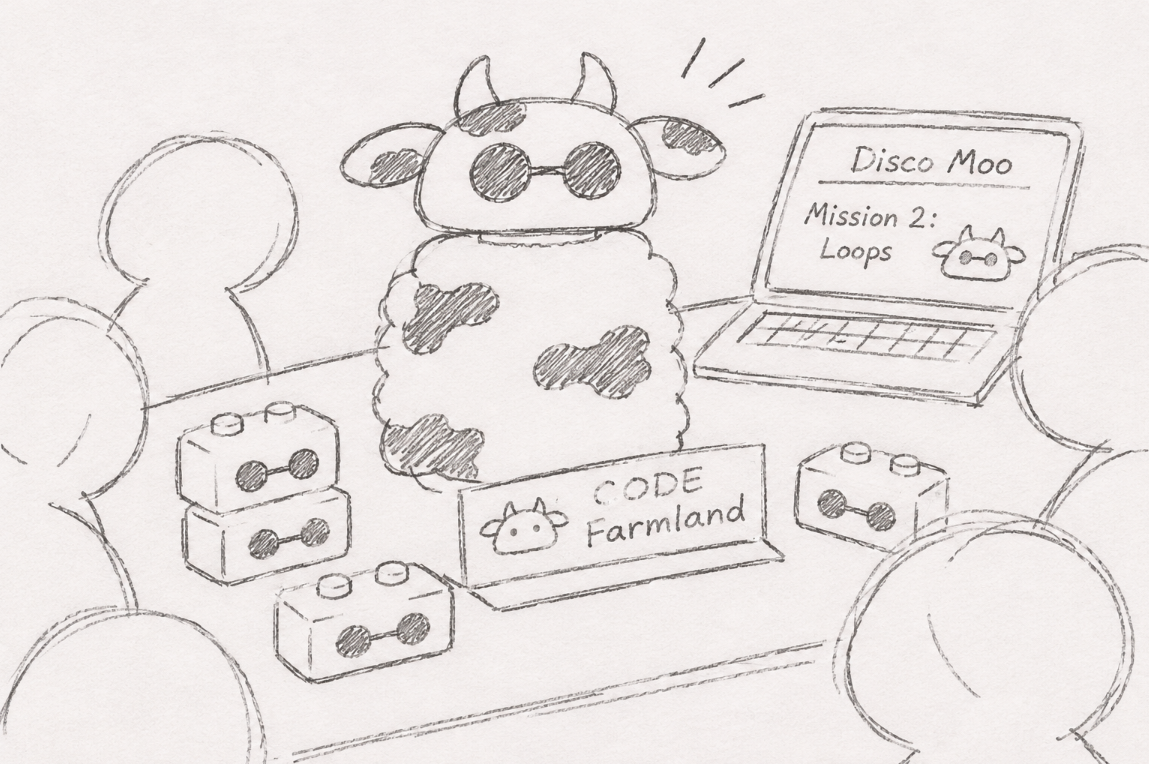
\includegraphics[width=\linewidth]{game_setting.png}
\caption{Proposed CODE Farmland setting with Reachy Mini, physical coding blocks, a shared display, and 3--4 collaborating students.}
\label{fig:setting}
\end{figure}

\section{Robot Control Architecture}

\subsection{Architecture Design}

In \emph{Moo-d Lab: The Emotion Factory}, Reachy's reply is produced by a student-triggered finite-state machine. The implemented states are READY, SCANNING, SHOWING\_SEQUENCE, RUNNING, CELEBRATING, and ERROR. From READY, the display shows the robot's camera while the group plans. SCANNING captures one frame when a student presses Scan. A stack whose markers all belong to the gesture registry passes through SHOWING\_SEQUENCE, which lists the program, and RUNNING, which plays each gesture while the active line is highlighted. CELEBRATING then runs a short fixed ending and returns to READY. A missing frame, an empty view, an unrecognized marker, or a motion fault enters ERROR, the robot stays still or stops at the failed step, and the group may scan again.

The machine is hybrid. At scan time it makes one discrete decision, accepting the whole stack or rejecting it. After acceptance, playback is an open sequence of predefined poses. The outer loop closes through the group. The webpage gives one student, the Actor, a short social scenario; the Actor performs it; the other students stack gesture blocks as Moo's response. Reachy embodies that stack, the Actor reacts, and the webpage carries the story forward from the completed performance. The group may restack and rescan. A greeting, a happy dance, or a reassuring reply is fixed by the scenario and by the blocks the group chooses. The controller makes that order visible and then performs it.

\subsection{Implementation Details}

The scanner opens a network connection to the Reachy Mini daemon, enables the motors, and settles to a neutral pose. Automatic body yaw is disabled, so a head turn and a body twist stay independent commands. On each Scan, OpenCV reads ArUco markers from dictionary \texttt{DICT\_6X6\_250} in that single frame and orders them from the top of the image to the bottom. The top block is the first gesture. Two copies of the same marker remain two steps, so a repeated feeling is programmed by stacking the same block again.

Marker IDs 10--16 are the vocabulary: look left, look right, nod, shake head, wiggle antennas, twist body left, and twist body right. Each ID resolves to a student-facing label, a line of display syntax, and an action key. Students read the syntax on screen. The action key selects a handler that sends a short chain of \texttt{goto\_target} poses. Each pose lasts at least 0.5\,s and blocks until the SDK reports that the move has finished. Commanded angles stay inside the conservative limits carried forward from earlier labs: head yaw and pitch within $18^{\circ}$, antennas within 0.50\,rad, and body yaw within 0.20\,rad. An unknown or empty stack is turned away before the first pose.

Every accepted program ends with the same celebration: the antennas sweep, the head nods, and the robot returns to neutral. The controller appends this dance after the last student block, which gives each social reply a shared closing beat. The on-screen list, with the current step highlighted, is the visual feedback for the group. A companion webpage can take that completed program, together with the Actor's reaction, as the cue for the next story beat. Scenario text, reaction choices, and prerecorded sounds live on that page. Joining the page to the scanner is the remaining integration; the scan-and-play cycle is already implemented.

\subsection{Level of Autonomy}

After Scan, detection, ordering, acceptance, on-screen playback, motor execution, and the celebration proceed on their own. Scan stays disabled until the cycle returns to READY or ERROR. A facilitator opens the session, confirms the connection, and can recover from a fault. The Actor's scene and the group's planning are human turns around this cycle. Any facilitator help with webpage transitions will be recorded apart from the autonomous scan-and-play behavior.

\subsection{Architecture Diagram}

Figure~\ref{fig:architecture} places the social turn around the implemented scan-and-play cycle. Students close the loop by revising the stack.

\begin{figure}[H]
\centering
\fbox{\parbox[c]{0.92\linewidth}{
\centering
\small
\textbf{Webpage scenario; Actor performs}\\
$\downarrow$\\
\textbf{Teammates stack a gesture reply}\\
$\downarrow$\\
\textbf{Scan: one frame from Reachy's camera}\\
$\downarrow$\\
\textbf{ArUco detection, top to bottom}\\
$\downarrow$\\
\textbf{Registry check (IDs 10--16); else ERROR, robot still}\\
$\downarrow$\\
\textbf{Show sequence, then play each action key}\\
$\downarrow$\\
\textbf{Fixed celebration, then READY}\\
$\downarrow$\\
\textbf{Actor reacts; webpage advances; group may rescan}
}}
\caption{Social turn around the implemented scan-and-play controller. The webpage and the Actor give the gesture sequence its story; the controller validates the stack and embodies it.}
\label{fig:architecture}
\end{figure}

\section{Robot Design and Prototyping}

\subsection{Robot Design and Form}

We used \emph{sketching, storyboarding, 3D printing, and laser cutting} to develop Disco Moo. Sketches explored character concepts; a storyboard mapped challenge presentation, role rotation, block assembly, scanning, execution, and debugging. The chosen cow persona makes mistakes feel like helping a character learn. Its soft spotted costume preserves Reachy's eyes, head motion, and antennas; modular blocks echo the robot's circular-eye motif.

\subsection{Fabrication and Materials}

A removable coat combines felt backing, white yarn, black yarn patches, hot glue, and adjustable retaining cords. Iteration replaced a poorly fitting flat wrap with a secure, removable fastening system that avoids blocking cameras, ventilation, or movement. Interlocking coding blocks were 3D-printed; socket tolerances of 14.00--14.03 mm were tested for fit. A 5 mm wooden CODE Farmland sign was laser-cut and engraved. These choices provide soft character embodiment, reusable physical commands, and a stable tabletop setting. Attaching readable ArUco labels to the blocks remains future work.

\section{User Studies}

\subsection{Procedure}

At the K--12 demonstration, groups of 3--4 students will play for 5--6 minutes, followed by 1--2 minutes of evaluation. \textbf{(1) Setup:} calibrate camera, test recognition, connectivity, and safe movements. \textbf{(2) Introduction:} explain the game and demonstrate a block. \textbf{(3) Roles:} assign and rotate Planner, Builder, Debugger, and Observer. \textbf{(4) Gameplay:} students assemble and scan programs; Reachy executes them. \textbf{(5) Feedback:} students receive condition-specific feedback and retry as needed. \textbf{(6) Evaluation:} collect learning responses and event-wide robot-perception measures. \textbf{(7) Reset:} restore blocks, interface, and robot position. Proposed team duties: Elliot---setup and guidance; Yifan---software; Jaclyn---facilitation; Jiaxin---questions and observations (subject to group confirmation).

\subsection{Game Testbed and Pre-study Setup}

The testbed includes a stable table, cow-costumed Reachy, 8--12 blocks, sign, laptop, and marked scanning area. Before each group, we will check lighting, camera framing and marker visibility, motor limits, connection, and FSM reset. Recognition thresholds and movement timing will be calibrated during pilot tests; manual reset will handle failures. No ML model fine-tuning is required because ArUco detection uses predefined markers.

\subsection{Evaluation: Study Design}

\textbf{RQ1} will be studied through observed error categories, attempts, successful revisions, and group participation. For \textbf{H1}, groups will, if feasible, be assigned to \emph{A: specific encouraging hints} or \emph{B: neutral mismatch notifications}; missions and blocks remain identical. Feedback type is the independent variable; debugging success rate (corrected errors / error opportunities) is the primary dependent variable. Secondary outcomes include attempts, time to correction, and mission completion. Assignment is by group because students share a program. We will document prior coding experience and recognition failures, and interpret small samples descriptively.

\subsection{Evaluation: Measures}

Event-wide RoSAS~\cite{carpinella2017} and pre/post robot-perception questions assess warmth, competence, discomfort, and understanding of robots. Our three short educational items are:

\textbf{Q1 (sequencing):} What changes if LOOK RIGHT moves to the beginning of LOOK LEFT--NOD--LOOK RIGHT?

\textbf{Q2 (loops):} How can REPEAT 3 with NOD replace three NOD commands?

\textbf{Q3 (debugging):} If the target is LEFT--NOD--RIGHT but the robot does LEFT--RIGHT--NOD, what should be fixed?

Each response receives 1 point if correct, 0 otherwise (total 0--3). Equivalent pre/post items will be used if time permits; otherwise results are descriptive post-game evidence. Observation notes supplement scores. We will not infer long-term learning from a single short session.

\section{Materials and Supplies}

\subsection{Materials for Game Components}

We will reuse one Reachy Mini, one removable cow costume, approximately 8--12 3D-printed blocks, one laser-cut sign, one computer, and printed ArUco labels. Blocks enable programming; the display shows missions and recognized sequences; costume and sign establish the setting.

\subsection{Budget and Justification}

No new purchases are currently required; existing Lab 4 prototypes, equipment, and lab printing resources will be reused. Any later supply needs will require approval within the \$20 cap.

\begin{table}[H]
\centering
\caption{Requested supplies and budget.}
\label{tab:budget}
\begin{tabularx}{\linewidth}{@{}p{0.32\linewidth}Y@{}}
\hline
\textbf{Field} & \textbf{Requested item}\\
\hline
Supply & Existing blocks, costume, sign, and lab resources\\
Justification & Reuse Lab 4 prototypes\\
Additional quantity & 0\\
Unit price (\$) & 0.00\\
Line total (\$) & 0.00\\
Purchase URL & N/A; no purchase required\\
\hline
Total request (\$) & 0.00\\
\hline
\end{tabularx}
\end{table}

\begin{thebibliography}{00}

\bibitem{paper1}
R. Sinha, H. Swanson, J. Clarke-Midura, J. F. Shumway, V. R. Lee, and S. Chandrasekharan,
``From Embodied Doing to Computational Thinking in Kindergarten: A Punctuated Motor Control Model,''
in \textit{Proc. ACM Symposium on Learning, Design and Technology},
2023.
doi: 10.1145/3594781.3594794.

\bibitem{paper2}
C. De Jong, J. Peter, R. K\"uhne, and A. Barco,
``Children's Acceptance of a Domestic Social Robot: How It Evolves over Time,''
\textit{ACM Transactions on Human-Robot Interaction},
vol. 13, no. 2, art. 17, 2024.
doi: 10.1145/3638066.

\bibitem{paper3}
M. E. U. Ligthart, S. M. De Droog, M. Bossema, L. Elloumi,
M. de Haas, M. H. J. Smakman, K. V. Hindriks, and S. Ben Allouch,
``Back to School---Sustaining Recurring Child-Robot Educational Interactions After a Long Break,''
in \textit{Proc. ACM/IEEE International Conference on Human-Robot Interaction},
2024, pp. 433--442.
doi: 10.1145/3610977.3635001.

\bibitem{paper4}
A. Misirli and V. Komis,
``Computational thinking in early childhood education: The impact of programming a tangible robot on developing debugging knowledge,''
\textit{Early Childhood Research Quarterly},
vol. 65, pp. 139--158, 2023.
doi: 10.1016/j.ecresq.2023.05.014.

\bibitem{carpinella2017}
C.~M. Carpinella, A.~B. Wyman, M.~A. Perez, and S.~J. Stroessner,
\emph{The Robotic Social Attributes Scale (RoSAS): Development and validation},
in \textit{Proc. ACM/IEEE International Conference on Human-Robot Interaction},
2017, pp.~254--262. doi: 10.1145/2909824.3020208.

\end{thebibliography}

\end{document}
